%\VignetteIndexEntry{Analyzing metagenomic data with metagenomeSeq}
\documentclass[a4paper,12pt]{article}
\usepackage{Sweave}
\usepackage{url}
\usepackage{afterpage}
\usepackage{hyperref}
\usepackage{geometry}
\usepackage{cite}
\geometry{hmargin=2.5cm, vmargin=2.5cm}
\usepackage{graphicx}
\usepackage{courier}
\bibliographystyle{unsrt}

\begin{document}
\Sconcordance{concordance:metagenomeSeq.tex:metagenomeSeq.Rnw:%
1 26 1 1 7 41 1 1 2 1 0 3 1 6 0 1 2 3 1 1 3 %
2 0 1 2 4 0 1 2 4 1 1 2 1 0 3 1 14 0 1 2 9 1 %
1 2 1 0 1 1 13 0 1 2 4 1 1 2 1 0 2 1 9 0 1 2 %
3 1 1 2 1 0 1 1 1 2 24 0 1 2 9 1 1 2 1 0 1 1 %
3 0 1 2 2 1 1 2 7 0 1 2 12 1 1 2 1 0 1 1 3 0 %
1 2 2 1 1 2 1 0 1 1 23 0 1 2 1 4 35 1 1 2 1 %
0 5 1 6 0 1 2 4 1 1 2 1 0 4 1 15 0 1 2 11 1 %
1 4 3 0 1 1 19 0 1 2 8 1 1 2 1 0 1 1 1 2 1 0 %
1 2 4 0 1 2 9 1 1 2 26 0 6 1 1 2 1 0 2 1 3 0 %
1 2 1 1 1 2 1 0 1 2 1 0 2 1 3 0 1 2 13 1 1 2 %
28 0 1 2 1 1}

\title{{\textbf{Analyzing metagenomic data with \texttt{metagenomeSeq}}}}
\author{Joseph Nathaniel Paulson\\[1em]\\ Center for Bioinformatics and Computational Biology\\ University of Maryland, College Park\\[1em]\\ \texttt{jpaulson@umiacs.umd.edu}}
\date{March 11, 2013}
\maketitle
\tableofcontents

\newpage


\section{Introduction}

Metagenomics is the study of genetic material targeted directly from an environmental community. 
Originally focused on exploratory and validation projects, these studies now focus on understanding the differences in microbial communities caused by phenotype differences. 
Analyzing high-throughput sequencing data has been a challenge to researchers due to the unique biological and technological biases that are present in marker-gene survey data.

 We present a R package, \texttt{metagenomeSeq} (metagenomic analysis in R), that implements methods developed to account for previously unaddressed biases specific to high-throughput sequencing marker-gene survey data.
Metastats \cite{metastats} and Lefse \cite{lefse} 
 are two statistical methods addressing differential abundance detection in clinical metagenomic datasets. 
 White \textit{et al.}'s Metastats used a non-parametric permutation test on $t$-statistics and Segata \textit{et al.}'s Lefse used a non-parametric Kruskal-Wallis test followed by subsequent wilcox rank-sum tests on subgroups to guard against positive discoveries of differential abundance driven by potential confounders.

This vignette is meant to describe the software package \texttt{metagenomeSeq}. 
A normalization method is implemented to control for biases in measurements across taxanomic features. 
We use a mixture model that implements a zero-inflated Gaussian distribution to account for varying depths of coverage. 
Using a linear model methodology, it is easy to include confounding sources of variability and interpret results. 
Additionally, visualization functions are provided to examine discoveries. 

The software was designed to determine features (be it Operational Taxanomic Unit (OTU), species, etc.) that are differentially abundant between two or more groups of multiple samples. 
The software was also designed to address the effects of both normalization and under-sampling of microbial communities on disease association detection and testing of feature correlations.

\section{Data structure}

Microbial marker gene sequence data is preprocessed and counts are algorithmically defined from project-specific sequence data by clustering reads according to read similarity. 
Given $m$ features and $n$ samples, the elements in a count matrix \textbf{C} ($m, n$), $c_{ij}$, are the number of reads annotated for a particular feature $i$ (whether it be OTU, species, genus, etc.) in sample $j$.

The S4 class system in R allows for object oriented definitions. \texttt{metagenomeSeq} makes use of the \texttt{Biobase} package in Bioconductor and their virtual-class, \texttt{eSet}. Building off of \texttt{eSet}, the main S4 class in \texttt{metagenomeSeq} is termed \texttt{MRexperiment}. \texttt{MRexperiment} is a simple extension of \texttt{eSet}, adding a single slot, \texttt{expSummary}. Experiment summary is a data frame that includes the depth of coverage and the normalization factors for each sample. Future datasets can be formated as MRexperiment objects and analyzed with relative ease. A \texttt{MRexperiment} object is created by calling \texttt{newMRexperiment}, passing the counts, phenotype and feature data as parameters.

We do not include normalization factors or library size in the currently available slot specified for the sample specific phenotype data. As expected, all matrices are organized in the \texttt{assayData} slot. All phenotype data (disease status, age, etc.) is stored in \texttt{phenoData} and feature data (OTUs, taxanomic assignment to varying levels, etc.) in \texttt{featureData}. Additional slots are available for reproducibility and annotation.

\subsection{Loading count and meta data}

Following preprocessing and annotation of sequencing data the easiest way to format the count matrix is to have features 
(be it OTU, species, genus, etc.) along rows and samples along the columns.
\texttt{metagenomeSeq} includes functions for loading delimited files of counts 
\texttt{load$\_$meta} and phenodata \texttt{load$\_$phenoData}.

As an example, a portion of the lung microbiome \cite{charlson} OTU matrix is provided in \texttt{metagenomeSeq}'s library "extdata" folder. 
The OTU matrix is stored as a tab delimited file.
\texttt{load\_meta} loads the taxa and counts into a list.

\begin{small}
\begin{Schunk}
\begin{Sinput}
R> library(metagenomeSeq)
R> dataDirectory <- system.file("extdata", package="metagenomeSeq")
R> lung = load_meta(file.path(dataDirectory,"CHK_NAME.otus.count.csv")) 
R> dim(lung$counts)
\end{Sinput}
\begin{Soutput}
[1] 1000   78
\end{Soutput}
\end{Schunk}
\end{small}
Next we want to load the annotated taxonomy. Check to make sure that your taxa annotations and OTUs are in the same order as your matrix rows.

\begin{small}
\begin{Schunk}
\begin{Sinput}
R> taxa = read.csv(file.path(dataDirectory,"CHK_otus.taxonomy.csv"),
                 sep="\t",header=T,stringsAsFactors=F)[,2]
R> otu  = read.csv(file.path(dataDirectory,"CHK_otus.taxonomy.csv"),
                 sep="\t",header=T,stringsAsFactors=F)[,1]
\end{Sinput}
\end{Schunk}
\end{small}

As our OTUs appear to be in order with the count matrix we loaded earlier, the next step is to load phenodata. Phenotype data can be optionally loaded into \texttt{R} with \texttt{load\_phenoData}. This function loads data as a list. It is important to properly order data.

\begin{small}
\begin{Schunk}
\begin{Sinput}
R> clin = load_phenoData(file.path(dataDirectory,"CHK_clinical.csv"),tran=TRUE)
R> ord = match(colnames(lung$counts),rownames(clin)) 
R> clin = clin[ord,]
R> head(clin[1:2,])
\end{Sinput}
\begin{Soutput}
                                         SampleType
CHK_6467_E3B11_BRONCH2_PREWASH_V1V2 Bronch2.PreWash
CHK_6467_E3B11_OW_V1V2                           OW
                                             SiteSampled
CHK_6467_E3B11_BRONCH2_PREWASH_V1V2 Bronchoscope.Channel
CHK_6467_E3B11_OW_V1V2                        OralCavity
                                    SmokingStatus
CHK_6467_E3B11_BRONCH2_PREWASH_V1V2        Smoker
CHK_6467_E3B11_OW_V1V2                     Smoker
\end{Soutput}
\end{Schunk}
\end{small}

\subsection{Creating a \texttt{MRexperiment} object}

\texttt{Biobase} provides functions to create annotated data frames. 
phenoData and featureData inputs are required to be annotated data frames. 
Function \texttt{newMRexperiment} takes a count matrix, phenoData (annotated data frame), and featureData (annotated data frame) as input. 
Library sizes (depths of coverage) and normalization factors are also optional inputs.

\begin{small}
\begin{Schunk}
\begin{Sinput}
R> phenotypeData = as(clin,"AnnotatedDataFrame")
R> phenotypeData
\end{Sinput}
\begin{Soutput}
An object of class 'AnnotatedDataFrame'
  rowNames:
    CHK_6467_E3B11_BRONCH2_PREWASH_V1V2
    CHK_6467_E3B11_OW_V1V2 ...
    CHK_6467_E3B09_BAL_A_V1V2 (78 total)
  varLabels: SampleType SiteSampled
    SmokingStatus
  varMetadata: labelDescription
\end{Soutput}
\end{Schunk}
\end{small}

A taxa feature annotated data frame. In this example it is simply the OTU numbers, but it can as easily be the annotated taxonomy at multiple levels.

\begin{small}
\begin{Schunk}
\begin{Sinput}
R> OTUdata = as(lung$taxa,"AnnotatedDataFrame")
R> varLabels(OTUdata) = "taxa"
R> OTUdata
\end{Sinput}
\begin{Soutput}
An object of class 'AnnotatedDataFrame'
  rowNames: 1 2 ... 1000 (1000 total)
  varLabels: taxa
  varMetadata: labelDescription
\end{Soutput}
\end{Schunk}
\end{small}

Links to a paper providing further details can be included optionally.
\begin{small}
\begin{Schunk}
\begin{Sinput}
R> counts = lung$counts
R> obj = newMRexperiment(counts,phenoData=phenotypeData,featureData=OTUdata)
R> #experimentData(obj) = annotate::pmid2MIAME("21680950")
R> obj
\end{Sinput}
\begin{Soutput}
MRexperiment (storageMode: environment)
assayData: 1000 features, 78 samples 
  element names: counts 
protocolData: none
phenoData
  sampleNames:
    CHK_6467_E3B11_BRONCH2_PREWASH_V1V2
    CHK_6467_E3B11_OW_V1V2 ...
    CHK_6467_E3B09_BAL_A_V1V2 (78 total)
  varLabels: SampleType SiteSampled
    SmokingStatus
  varMetadata: labelDescription
featureData
  featureNames: 1 2 ... 1000 (1000 total)
  fvarLabels: taxa
  fvarMetadata: labelDescription
experimentData: use 'experimentData(object)'
Annotation:  
\end{Soutput}
\end{Schunk}
\end{small}


\section{Normalization}
Normalization is required due to variable depths of coverage. We have implemented in \texttt{cumNorm} a normalization method that calculates normalization factors automatically calculated as the sum of counts less than the percentile that the majority of sample counts deviate from a reference. These normalization factors are stored in the experiment summary slot. Functions to determine the proper percentile \texttt{cumNormStat}, save normalized counts \texttt{exportMat}, or save various sample statistics \texttt{exportStats} are also provided.
Normalized counts can be called easily by \texttt{cumNormMat(MRexperimentObject)} or \texttt{MRcounts(MRexperimentObject,norm=TRUE)}.

\subsection{Calculating normalization factors}
After defining a \texttt{MRexperiment} object, the first step is to calculate the proper percentile by which to normalize counts. There are several options in calculating and visualizing the relative differences in the reference. Figure 1 is an example for the longitudinal gnotobiotic mouse dataset.
\begin{small}
\begin{Schunk}
\begin{Sinput}
R> data(lungData)
R> p=cumNormStat(lungData)
\end{Sinput}
\end{Schunk}
\end{small}
To calculate the scaling factors we simply run \texttt{cumNorm}
\begin{small}
\begin{Schunk}
\begin{Sinput}
R> cumNorm(lungData,p=p)
\end{Sinput}
\begin{Soutput}
[1] TRUE
\end{Soutput}
\end{Schunk}
\end{small}

There are other functions, including \texttt{normFactors}, \texttt{cumNormMat}, that relatively extract the normalization factors and create a normalized matrix for a specified percentile. To see a full list of functions please see the manual and help pages. 

\begin{figure}
\centerline{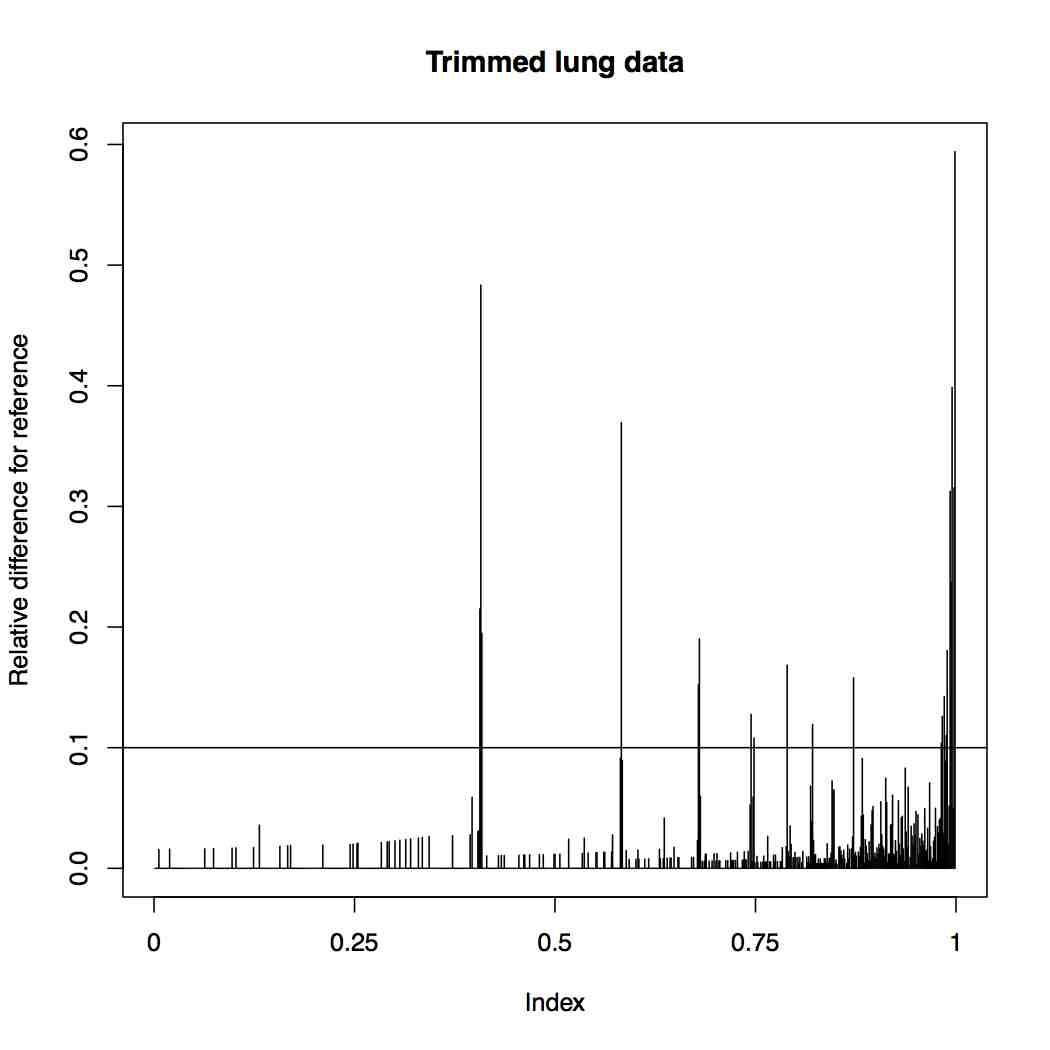
\includegraphics[width=.55\textwidth]{metagenomeSeq_figure1.png}\label{fig1}}
\caption{Relative difference for the median difference in counts from the reference. Samples came from the lung dataset (and all were used except the extraction.controls \texttt{pData(lungData)\$SampleType}). }
\end{figure}

\subsection{Exporting data}
Functions are provided to easily retrieve or save normalized count matrices or basic sample characteristic statistics.

\begin{small}
\begin{Schunk}
\begin{Sinput}
R> mat = MRcounts(lungData,norm=TRUE)[1:5,1:5]
R> exportMat(mat,output=file.path(dataDirectory,"temp.tsv"))
\end{Sinput}
\end{Schunk}
\end{small}

\begin{small}
\begin{Schunk}
\begin{Sinput}
R> exportStats(lungData[,1:5],output=file.path(dataDirectory,"temp.tsv"),p=p)
R> head(read.csv(file=file.path(dataDirectory,"temp.tsv"),sep="\t"))
\end{Sinput}
\begin{Soutput}
                              Subject
1 CHK_6467_E3B11_BRONCH2_PREWASH_V1V2
2              CHK_6467_E3B11_OW_V1V2
3              CHK_6467_E3B08_OW_V1V2
4           CHK_6467_E3B07_BAL_A_V1V2
5           CHK_6467_E3B11_BAL_A_V1V2
  Scaling.factor Quantile.value
1             36              4
2           2681              1
3           2390              1
4            897              1
5            802              2
  Number.of.features
1                 60
2               3299
3               2994
4               1188
5               1098
\end{Soutput}
\end{Schunk}
\end{small}

\section{Zero-inflated Gaussian mixture model}

The depth of coverage in a sample is directly related to how many features are detected in a sample motivating our zero-inflated Gaussian (ZIG) mixture model. Figure 2 is representative of the sparsity ubiquitous in marker-gene survey datasets currently available. 

Function \texttt{fitZig} performs a complex mathematical optimization routine to estimate probabilities that a zero for a particular feature in a sample is a technical zero or not. The function relies heavily on the \texttt{limma} package \cite{limma}.

\subsection{Mathematical model}

Defining the class comparison of interest as $k(j)=I\{j \in \mathrm{ group } A\}$. The zero-inflated model is defined for the continuity-corrected $\log_2$ of the count data $y_{ij} = \log_2(c_{ij}+1)$ as a mixture of a point mass at zero $I_{\{0\}}(y_{ij})$ and a count distribution $f_{count}(y_{ij};\mu_i, \sigma_i^2) \sim N(\mu_i, \sigma_i^2)$.
Given mixture parameters $\pi_{j}$, we have that the density of the zero-inflated Gaussian distribution for feature $i$, in sample $j$ with $s_{j}$ total counts is:

\begin{equation}
f_{zig}(y_{ij}; \theta ) = \pi_{j}(s_{j}) \cdot I_{\{0\}}(y_{ij})
+ (1-\pi_{j}(s_{j})) \cdot f_{count}(y_{ij};\theta)
\end{equation}

Maximum-likelihood estimates are approximated using an EM algorithm,
where we treat mixture membership $\Delta_{ij}=1$ if $y_{ij}$ is
generated from the zero point mass as latent indicator variables\cite{EM}.

Design matrices can be created in R by using the \texttt{model.matrix} function and are inputs for \texttt{fitZig}.

For large survey studies it is often pertinent to include phenotype information or confounders into a design matrix when testing the association between the abundance of taxonomic features and a phenotype phenotype of interest (disease, for
instance). Our linear model methodology can easily incorporate these
confounding covariates in a straightforward manner. \texttt{fitZig} output includes weighted fits for each of the $m$ features. Results can be filtered and saved using \texttt{MRcoefs} or \texttt{MRtable}. \texttt{MRfisher} tests assumptions different from the difference in abundance of a feature. Instead, it tests the odds of a feature being present or absent between two groups. 

\begin{figure}
\centerline{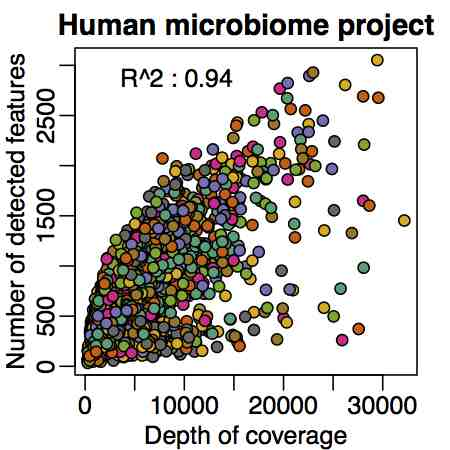
\includegraphics[width=.55\textwidth]{metagenomeSeq_figure2.png}}
\caption{The number of unique features is plotted against depth of coverage for samples from the Human Microbiome Project \cite{hmp}. Including the depth of coverage and the interaction of body site and sequencing site we are able to acheive an adjusted $\mathrm{R}^2$ of .94. The zero-inflated Gaussian mixture was developed to account for missing features.}\label{fig2}
\end{figure}

\subsection{Running the statistical analysis}
In our analysis of the lung microbiome data, we can remove features that are not present in many samples and samples that are controls and calculate the normalization factors. Following the calculation of our normalization factors the user needs to smartly decide/include pertinent phenotype parameters in a model matrix. 

\begin{small}
\begin{Schunk}
\begin{Sinput}
R> data(lungData)
R> k = grep("Extraction.Control",pData(lungData)$SampleType)
R> lungTrim = lungData[,-k]
R> k = which(rowSums(MRcounts(lungTrim)>0)<10)
R> lungTrim = lungTrim[-k,]
R> cumNorm(lungTrim)
\end{Sinput}
\begin{Soutput}
[1] TRUE
\end{Soutput}
\end{Schunk}
\end{small}

Following the preparation, the user must define a model matrix for the data. There are optional inputs to \texttt{fitZig}, including the settings found in \texttt{zigControl} and we ask the user to review the help files for both \texttt{fitZig} and \texttt{zigControl}. For this example we include body site as covariates and want to test for the bacteria differentially abundant between smokers and non-smokers.

\begin{small}
\begin{Schunk}
\begin{Sinput}
R> smokingStatus = pData(lungTrim)$SmokingStatus
R> bodySite = pData(lungTrim)$SampleType
R> mod = model.matrix(~smokingStatus+bodySite)
R> settings = zigControl(maxit=10,verbose=TRUE)
R> fit = fitZig(obj = lungTrim,mod=mod,control=settings)
\end{Sinput}
\begin{Soutput}
it= 0, nll=88.55, log10(eps+1)=Inf, stillActive=1029
it= 1, nll=93.10, log10(eps+1)=0.07, stillActive=299
it= 2, nll=93.24, log10(eps+1)=0.05, stillActive=130
it= 3, nll=93.47, log10(eps+1)=0.07, stillActive=31
it= 4, nll=93.49, log10(eps+1)=0.05, stillActive=15
it= 5, nll=93.50, log10(eps+1)=0.02, stillActive=9
it= 6, nll=93.52, log10(eps+1)=0.01, stillActive=5
it= 7, nll=93.52, log10(eps+1)=0.00, stillActive=2
it= 8, nll=93.52, log10(eps+1)=0.00, stillActive=1
it= 9, nll=93.52, log10(eps+1)=0.00, stillActive=0
\end{Soutput}
\end{Schunk}
\end{small}

The result, \texttt{fit}, is a list providing detailed estimates of the fits including a \texttt{limma} fit in \texttt{fit\$fit} and an \texttt{ebayes} statistical fit in \texttt{fit\$eb}. This data can be analyzed like any \texttt{limma} fit and in this example, the column of the fitted coefficients represents the fold-change for our "smoker" vs. "nonsmoker" analysis. 
Often we're interested in in the fold change of various features with respect to the a condition. Koch's postulates demand an increase in presence and abundance of a particular bacteria. As mentioned above, Fisher's test is implemented in \texttt{MRfisher} as a test for presence / absence test. This tests different assumptions of the 16S count data.

Looking at the particular analysis just performed, there appears to be OTUs representing three \textit{Prevotella}, two \textit{Neisseria}, and a \textit{Porphyromonas} that are differentially abundant.

It is important to check that similarly annotated OTUs are not equally differentially abundant in controls. 

Currently functions are being developed to wrap and output results more neatly, but \texttt{MRcoefs} and \texttt{MRfit} can be used to view coefficient fits and related statistics.

\begin{small}
\begin{Schunk}
\begin{Sinput}
R> taxa = 
   sapply(strsplit(as.character(fData(lungTrim)$taxa),split=";"),
          function(i){i[length(i)]})
R> head(MRcoefs(fit,taxa=taxa,coef=2))
\end{Sinput}
\begin{Soutput}
                            smokingStatusSmoker
Neisseria polysaccharea:1               -4.1303
Neisseria meningitidis:1                -3.9919
Prevotella intermedia:2                 -2.8587
Prevotella paludivivens:2                2.6978
Porphyromonas sp. UQD 414:2             -2.6957
Prevotella sp. DJF_B116:1                2.6458
                                pValue  adjPvalue
Neisseria polysaccharea:1   2.1379e-15 1.4666e-13
Neisseria meningitidis:1    2.0559e-14 1.1134e-12
Prevotella intermedia:2     9.1893e-12 2.7811e-10
Prevotella paludivivens:2   6.7642e-09 6.6092e-08
Porphyromonas sp. UQD 414:2 9.3234e-10 1.4109e-08
Prevotella sp. DJF_B116:1   1.2968e-10 2.6964e-09
\end{Soutput}
\end{Schunk}
\end{small}

\section{Visualization of features}
Reads clustered with high similarity do not represent functional or taxonomic units. It is possible that reads from the same organism get clustered into multiple OTUs. 
\texttt{metagenomeSeq} has several plotting functions to visualize abundance differences for a single feature, \texttt{plotOTU}, and multiple features \texttt{plotGenus}. 
Plotting multiple OTUs with similar annotations allows for additional control of false discoveries. Other functions allow for an understanding of structural composition with heatmaps of feature counts \texttt{plotMRheatmap} and basic feature correlation structures \texttt{plotCorr}.

Many studies hope to compare biological compositions at a community level. Often a first step of data analysis is a heatmap or some other data exploratory tool, followed by a correlation or co-occurence heatmap.
\begin{small}
\begin{Schunk}
\begin{Sinput}
R> data(mouseData)
R> trials = pData(mouseData)$diet
R> plotMRheatmap(obj=mouseData,n=200,trials=trials,
               cexRow = 0.4,cexCol = 0.4,trace="none")
R> plotCorr(obj=mouseData,n=200,
               cexRow = 0.25,cexCol = 0.25,trace="none",dendrogram="none")
\end{Sinput}
\end{Schunk}
\end{small}

\begin{figure}
\centerline{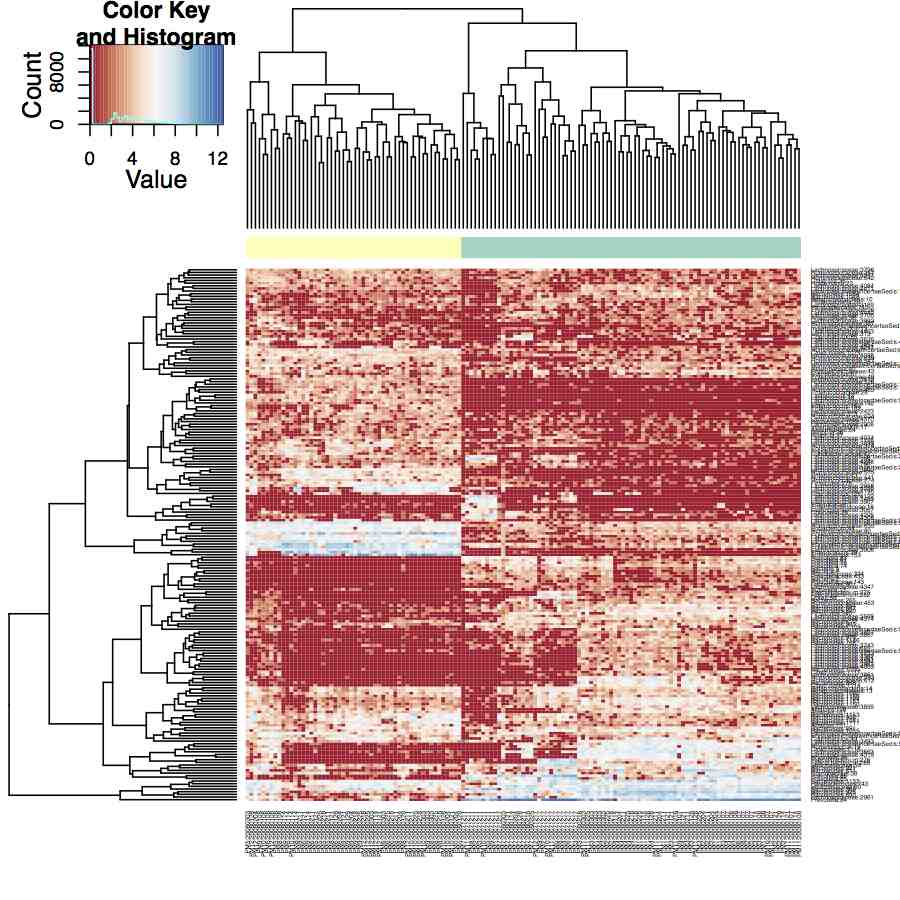
\includegraphics[width=.55\textwidth]{metagenomeSeq_figure3.png}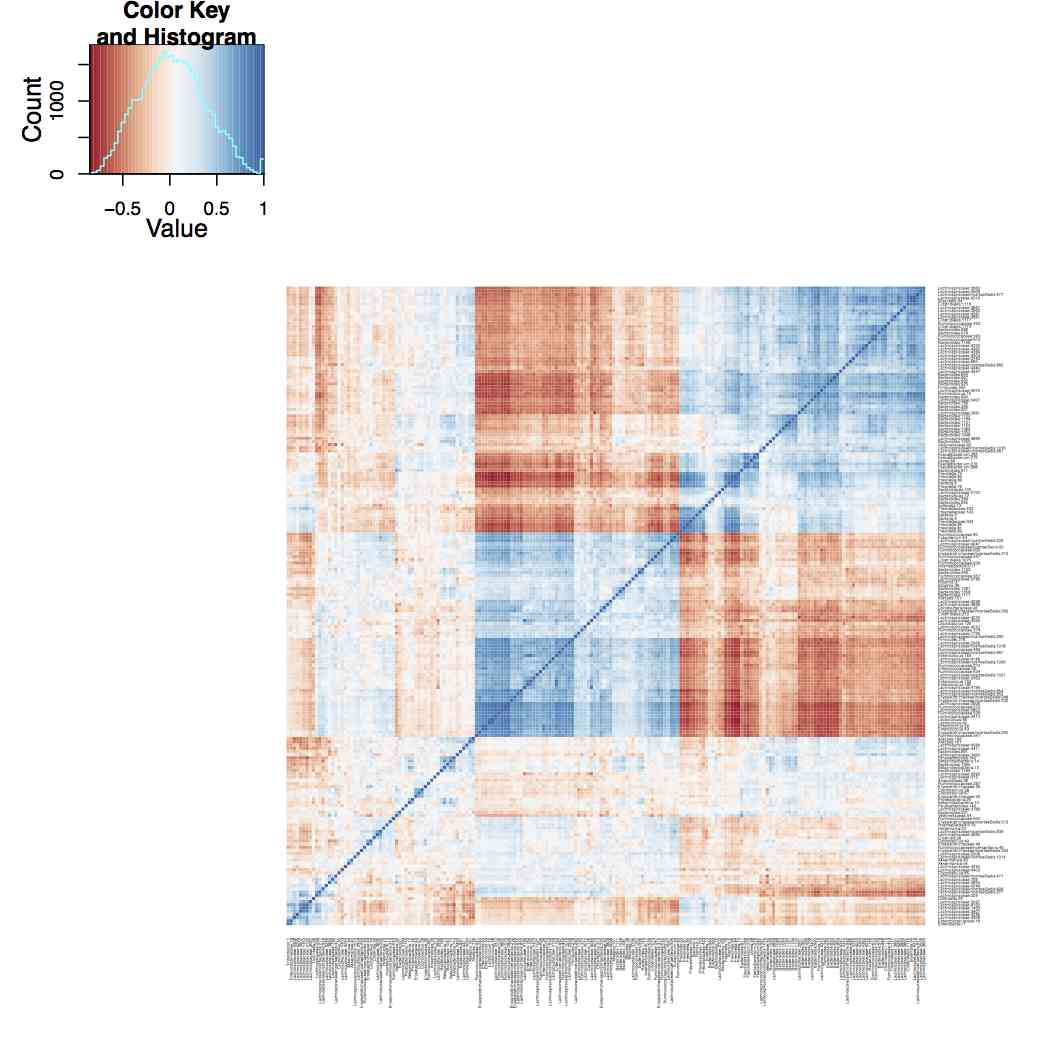
\includegraphics[width=.55\textwidth]{metagenomeSeq_figure4.png}\label{fig3}}
\caption{Left) Heatmaps and hierarchical clustering of log2 transformed counts for the 200 OTUs with the largest overall variance. Red values indicate counts close to zero. Row color labels indicate OTU taxonomic class; column color labels indicate diet (green = high fat, yellow = low fat). Notice the samples cluster by diet in these cases and there are obvious clusters. Right) Correlation matrix for the same features.}
\end{figure}

Following differential abundance analysis. It is important to confirm differential abundance. One way to limit false positives is ensure that the feature is actually abundant (enough positive samples). Another way is to plot the abundances of features similarly annotated. \texttt{plotOTU} allows the user to plot the abundances of one feature separately for one group versus another.

\begin{small}
\begin{Schunk}
\begin{Sinput}
R> head(MRtable(fit,coef=2,taxa=1:length(fData(lungTrim)$taxa)))
\end{Sinput}
\begin{Soutput}
      +samples in group 1 +samples in group 0
63:1                    6                  24
779:1                   7                  23
358:1                   1                  24
25:1                   26                  15
499:1                   2                  21
21:1                   23                  14
      counts in group 1 counts in group 0
63:1                 11              1538
779:1                22              1512
358:1                 1               390
25:1               1893               162
499:1                 2               326
21:1               1447               331
      smokingStatusSmoker     pValue  adjPvalue
63:1              -4.1303 2.1379e-15 1.4666e-13
779:1             -3.9919 2.0559e-14 1.1134e-12
358:1             -2.8587 9.1893e-12 2.7811e-10
25:1               2.6978 6.7642e-09 6.6092e-08
499:1             -2.6957 9.3234e-10 1.4109e-08
21:1               2.6458 1.2968e-10 2.6964e-09
\end{Soutput}
\begin{Sinput}
R> patients=sapply(strsplit(rownames(pData(lungTrim)),split="_"),function(i){i[3]})
R> pData(lungTrim)$patients=patients
R> classIndex=list(controls=which(pData(lungTrim)$SmokingStatus=="Smoker"))
R> classIndex$cases=which(pData(lungTrim)$SmokingStatus=="NonSmoker")
R> otu = 779
R> x = fData(lungTrim)$taxa[otu]
R> plotOTU(lungTrim,otu=otu,classIndex,xaxt="n",
         ylab="Normalized log(cpt)",main="Neisseria meningitidis")
R> lablist<- c("Smoker","NonSmoker")
R> axis(1, at=seq(1,2,by=1), labels = lablist)
\end{Sinput}
\end{Schunk}
\texttt{plotGenus} allows the user to plot abundances for several features similarly annotated for the various groups. At the OTU level reads are potentially clustered to multiple cluster centers that represent the same organism. It is possible that reads from one group get assigned to one OTU, and reads from another group are assigned to a different center that represents the same organism simply due to read similarity. Using \texttt{plotGenus} is one basic method to ensure that a feature is more likely to be differentially abundant.

\begin{Schunk}
\begin{Sinput}
R> otulist = grep(x,fData(lungTrim)$taxa)
R> plotGenus(lungTrim,otulist,classIndex,xaxt="n",
           ylab="Normalized log(cpt)",main="Neisseria meningitidis")
R> lablist<- c("S","NS")
R> axis(1, at=seq(1,6,by=1), labels = rep(lablist,times=3))
\end{Sinput}
\end{Schunk}


\begin{figure}
\centerline{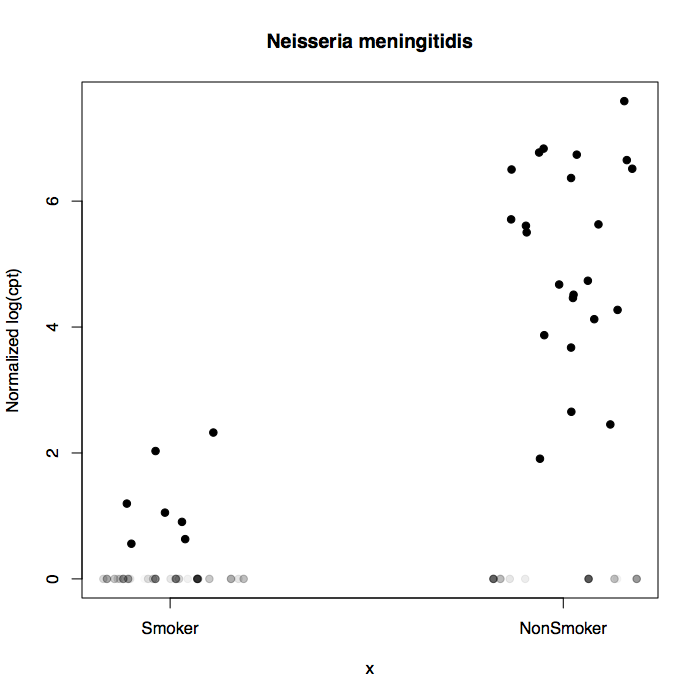
\includegraphics[width=.55\textwidth]{metagenomeSeq_figure5.png}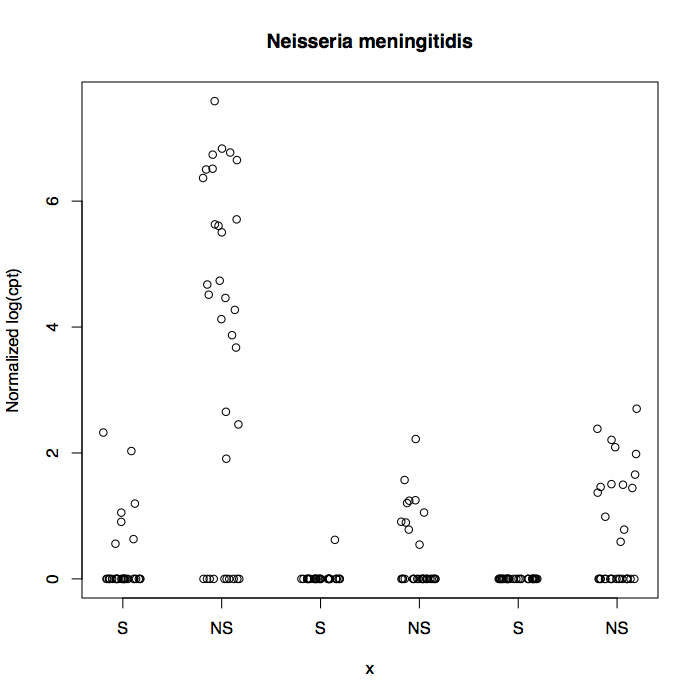
\includegraphics[width=.55\textwidth]{metagenomeSeq_figure6.png}\label{fig4}}
\caption{Left) Plot of the normalized log(cpt) of \textit{Neisseria meningitidis}, in particular the 779th row of lungTrim's count matrix. Right) Plot of the normalized log(cpt) of all OTUs annotated as \textit{Neisseria meningitidis}. According to this it would appear that \textit{Neisseria meningitidis} is differentially abundant and more abundant in nonsmokers.}
\end{figure}

\end{small}

\section{Summary}

\texttt{metagenomeSeq} is specifically designed for sparse high-throughput sequencing experiments that addresses the analysis of differential abundance for marker gene survey data. The package, while designed for marker-gene survey datasets, may be appropriate for other sparse data sets for which the zero-inflated Gaussian mixture model may apply.

\section{Session Info}
\begin{Schunk}
\begin{Sinput}
R> sessionInfo()
\end{Sinput}
\begin{Soutput}
R version 2.15.2 (2012-10-26)
Platform: x86_64-apple-darwin9.8.0/x86_64 (64-bit)

locale:
[1] en_US.UTF-8/en_US.UTF-8/en_US.UTF-8/C/en_US.UTF-8/en_US.UTF-8

attached base packages:
[1] grid      stats     graphics  grDevices
[5] utils     datasets  methods   base     

other attached packages:
 [1] metagenomeSeq_0.99.0 gplots_2.11.0       
 [3] MASS_7.3-23          KernSmooth_2.23-8   
 [5] caTools_1.14         gdata_2.12.0        
 [7] gtools_2.7.0         RColorBrewer_1.0-5  
 [9] matrixStats_0.6.2    limma_3.14.4        
[11] Biobase_2.18.0       BiocGenerics_0.4.0  

loaded via a namespace (and not attached):
[1] bitops_1.0-4.2    R.methodsS3_1.4.2
[3] tools_2.15.2     
\end{Soutput}
\end{Schunk}
\bibliography{metagenomeSeq}
\end{document}
